\documentclass[oneside, 12 pt]{book}
\usepackage{amsmath, amssymb}
\DeclareMathOperator*{\argmax}{argmax}

\usepackage[english]{babel}
\usepackage{microtype} %Tidyness
\usepackage{dsfont} %math 1
\usepackage[left = 4cm, right = 2.5cm, top = 2.5cm, bottom = 2.5cm]{geometry} %% Margin width
\linespread{1.5}
\usepackage{subfig} %% side by side figures
\usepackage{algpseudocode}
\usepackage{textcomp}
\usepackage{eurosym} %eurosymbol
\usepackage{graphicx}
\setcounter{secnumdepth}{4} %numbering for subsubsection 
\usepackage[Sonny]{fncychap} %Chapter Titles
\usepackage{afterpage} %spacing before landscape
\usepackage[version=3]{mhchem} % For Ca^2+
\let\oldemptyset\emptyset % empty set symbol
\usepackage{bbm} % for \mathbbm{}
\usepackage{bm}
\usepackage{mathtools} % for \splitdfrac{}
\usepackage[ruled,vlined]{algorithm2e}
%Add line numbers
 \usepackage{lineno}
\linenumbers


\begin{document}
\section{Mixing issues with the GP and resolutions}
%Current method
We currently use an under-relaxed method to propose new intensity functions when we assume the intensity has a Gaussian Process (GP) prior. In the under relaxed method the candidate intensity function $\mathbf{x}^*$ is composed of the current intensity function $\mathbf{x}$ and a draw from the GP prior $\nu$, namely  
\begin{equation}\label{eq:GPpropose}
\log \mathbf{x}^* = \sqrt{1-\omega^2} \log (\mathbf{x} ) + \omega \boldsymbol{\nu}, 
\qquad \qquad \boldsymbol{\nu} \sim \mathcal{N}(\mathbf{0}, \Sigma),
\end{equation}
where $\omega$ is a step size parameter.
% Problem with current method Example
However, we found that this method struggles to capture the behaviour of the intensity before the first spike and after the last spike. In particular, in these regions the posterior distribution of the intensity function often contains a peak in intensity at either time $0$ or at $T$ ---the end of experiment time --- or both.  
\begin{figure}[b!]
   \hrulefill
   \begin{center} 
    \subfloat{{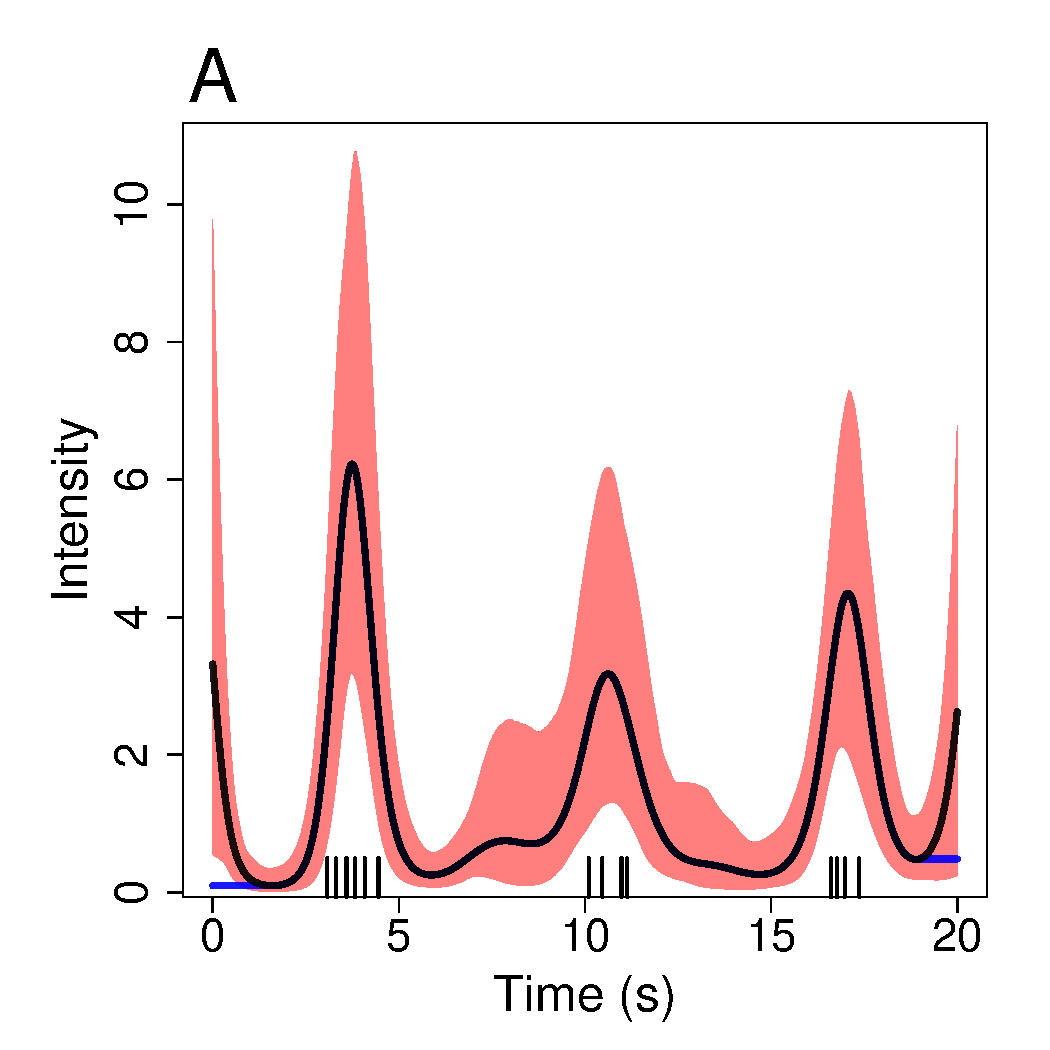
\includegraphics[width = 0.48\linewidth]{example.pdf} }}
      \subfloat{{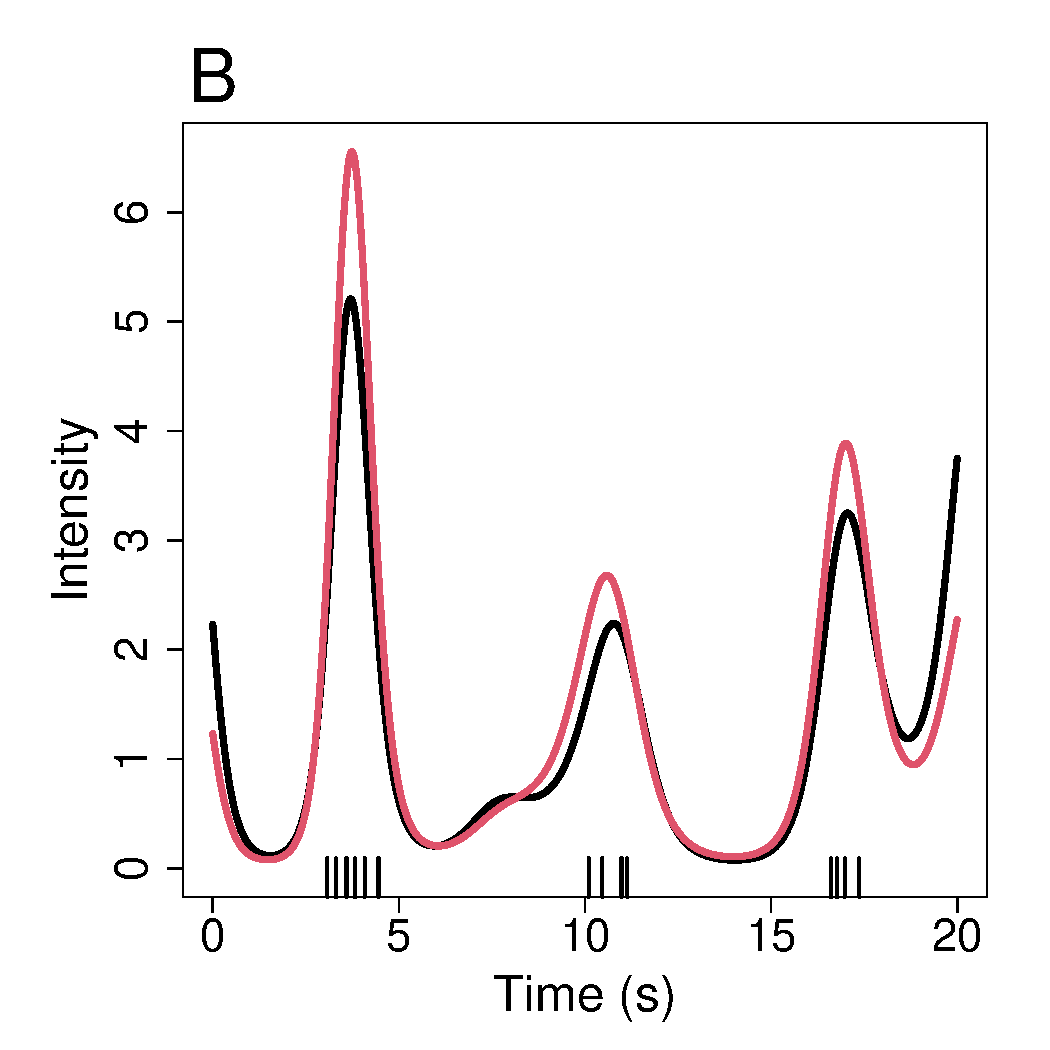
\includegraphics[width = 0.48\linewidth]{example2.pdf} }}
    \end{center}     
    \caption{(A) Posterior mean --- black line --- and 95\% confidence interval --- red shaded area --- for the intensity function. The blue line shows an altered version of the posterior mean which is flat in $[0,1.5]$ and $[19,20]$  (B) Two consecutive iterations from the MCMC calculation. The black ticks show the spike times used to infer the intensity function.}
    \label{fig:ExampleProb}
    \end{figure}
For example in Figure \ref{fig:ExampleProb}(A) we show the posterior distribution of the intensity function given a \ce{Ca^2+} spike sequence --- shown as black ticks --- where we assume a GP prior and a Gamma ISI distribution. The inference was calculated using $80000$ iterations after the initial $50000$ were binned, where time was discretised into $2000$ steps, the GP hyper parameters were   set to $\sigma_f^2 = 1000$, $\sigma_n^2 = 1e^{-5}$, $l=1.59$, the under-relaxed parameter $\omega = 0.001$ and the prior for the ISI parameter was an exponential with rate $0.01$. We see that the posterior intensity distribution captures the three peaks in intensity where the \ce{Ca^2+} spikes occur. Furthermore, we see that the intensity does decrease before the first peak and after the last peak in intensity --- approximately at the times $[1.6,3.7]$ and $[17,19]$. However, we also find large values of intensity at times $0$s and $20$s. Since there are no spikes close to these times you would expect the intensity to be close to zero. To quantify if our posterior distribution should have these regions of high intensity we compare the posterior mean with an altered version where the intensity is flattened in regions $[0,1.5]$ and $[19,20]$ --- shown in blue in Figure \ref{fig:ExampleProb}. We found that the log likelihood of the posterior mean is $-8.90$ and the altered version is $-7.20$. Therefore, we find that there is higher probability of these regions being flat. 
     
  
%Justification of problem
The problem in posterior computation lies in the mixing of the under-relaxed method. Since the candidate intensity varies over all time the change in one region may outweigh a change in another region. In particular,  in Figure \ref{fig:ExampleProb}(B) we give an example of an iteration where the current intensity function $\mathbf{x}$ is shown by the red line and the candidate intensity function $\mathbf{x^*}$ by the black line. We see that in $[0,1]$ and $[19,20]$ $\mathbf{x^*}$ is much greater than $\mathbf{x}$. However,  $\mathbf{x^*}$ is smaller that $\mathbf{x}$ in the three peaks --- at times $4$s, $10$s and $17$s --- which is closer to the underlying rate. Therefore we find the log likelihood of $\mathbf{x}$ is $-8.13$ and $\mathbf{x^*}$ is $-7.78$. Therefore, we would accept the candidate function. Moreover, once the features in $[0,1]$ and $[19,20]$ are accepted they are difficult to remove since a candidate function is likely to perform poorly in other regions of the function.
% Description of what we want to do.
Therefore, we want to create a new proposal mechanism to work in tandem with the under-relaxed method to improve the mixing at the beginning and end of the intensity function. We will do this by proposing candidate intensity functions that vary only on these regions of interest. In particular, we will call the proposals the conditional method at the start and conditional method at the end, for the proposals that only change values in the beginning of the experiment and end of experiment respectively.



\subsection{Method}
We begin by updating the intensity function only at the beginning of the function. Assume initially that we have discretised time into $N+1$ steps by $\mathbf{t} = \{t_0, t_1, \dots, t_N\}$ defined as $t_i = iT/N$ for $i \in \{0, \dots, N\}$. Furthermore, the current value of the discretised intensity function is $\mathbf{x} = \{x_0, \dots, x_N\}$ where $x_i =x(t_i)$ for $i \in \{0, \dots, N\}$. We need to decide how to partition $\mathbf{x}$ into two regions --- the part we update and the part that remains unchanged. We choose to sample the partition value uniformly between time zero and just after the first spike time. We do this because this region is where the under-relaxed method has difficulties mixing. Suppose the first spike occurs at time $t_\iota$, where $\iota \in \{1,\dots, N\}$. Then the partition value $M$ is drawn uniformly from the set $\{1,2, \dots, \min(\iota + w,N) \}$, where $w$ controls how far past the first spike we can sample. The minimum is used to only allow valid index values. We split time into two groups; one either side of $t_{M}$ --- $A = \{t_0, \dots t_{M}\}$ and $B = \{t_{M +1}, \dots t_N\}$. We similarly split the $\mathbf{x}$ into two groups $\mathbf{x}_A = \{x_0, \dots, x_{M}\}$ and $\mathbf{x}_B = \{x_{M +1}, \dots, x_{N}\}$. Therefore, the candidate intensity function $\mathbf{x}^\star$ consists of two parts: $\mathbf{x}^\star_A$  describing the new values we propose in region $A$ and $\mathbf{x}^\star_B$ which corresponds to the unchanged values in region $B$, $\mathbf{x}^\star_B$ =$\mathbf{x}_B$.


%Figure shows the splitting into A and B. 
  \begin{figure}[t]
   \hrulefill
   \begin{center} 
    \subfloat{{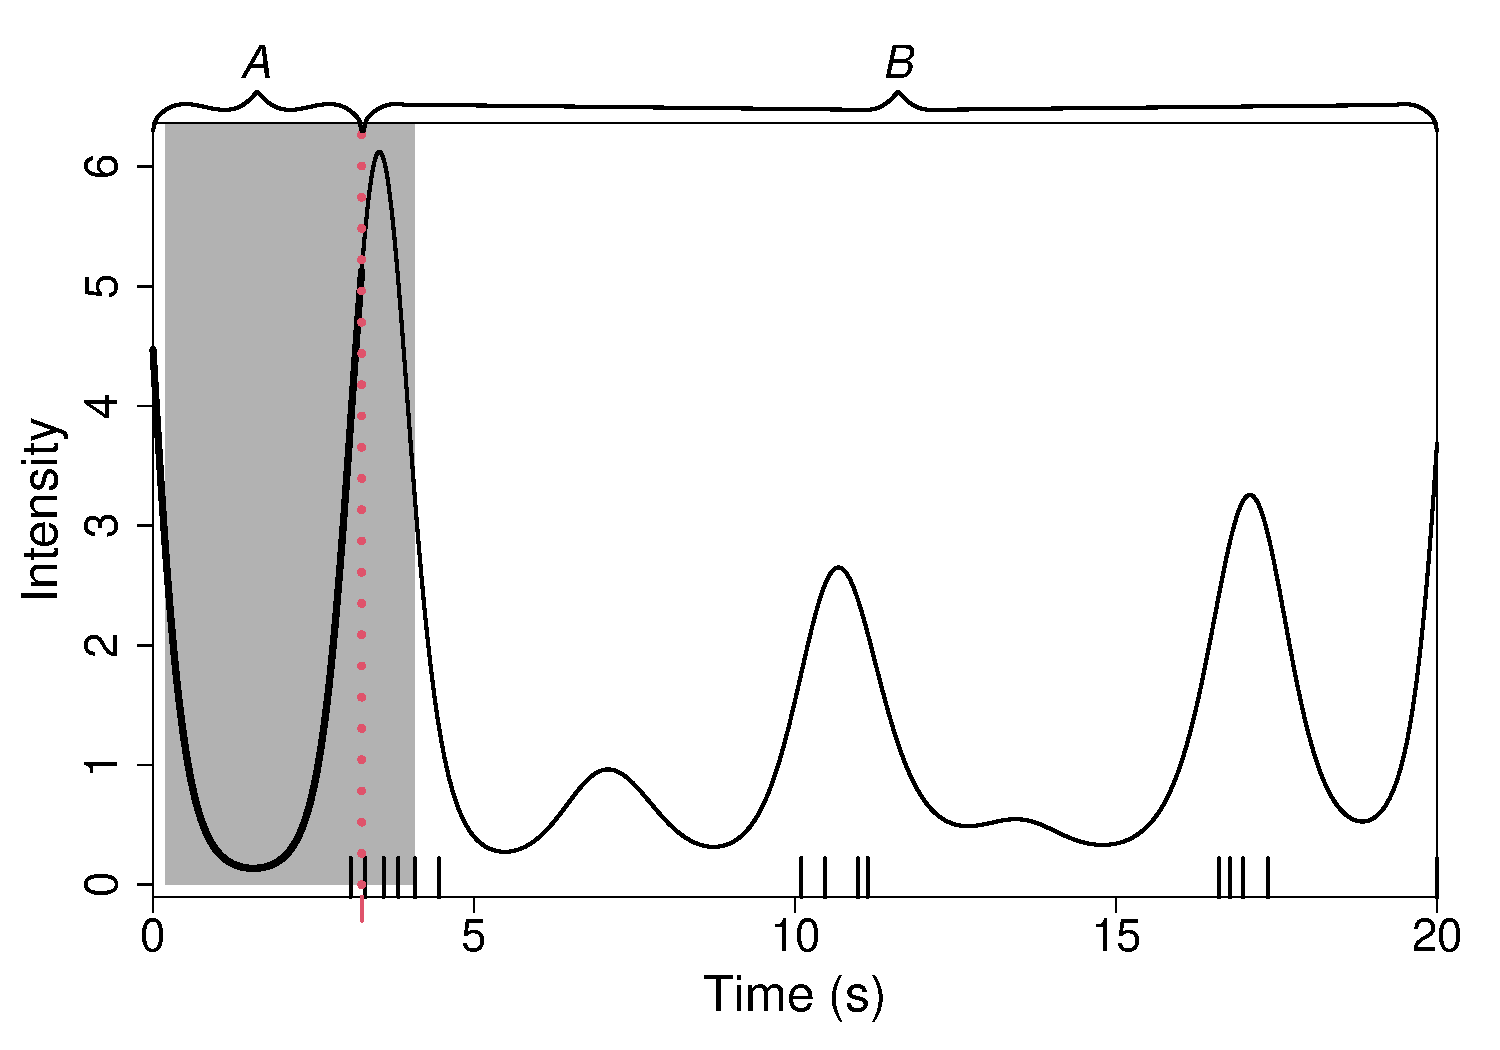
\includegraphics[scale = 0.55]{Proposal_1.pdf} }}
    \end{center}     
    \caption{Illustration of how to partition $\mathbf{x}$ into two regions $A$ and $B$. The partition value is drawn from the grey region. An example draw $t_M$ is shown by the dotted red line. The thick black line --- left of $t_M$ --- is the region of $\mathbf{x}$  we will propose new values for, whereas the thin black line --- right of $t_M$ --- will remain unchanged. The black ticks on the x-axis represent spike times.}
    \label{fig:Proposal1}
    \hrulefill
    \end{figure}
    
 %Describe the figure. 
 In Figure \ref{fig:Proposal1} we give an example of splitting $\mathbf{x}$ --- the black line --- into two regions. In this example $\mathbf{x}$ is discretised into $2000$ steps. The first spike occurs at $3.08$s which corresponds to the $308$th element of $\mathbf{t}$. Taking $w = 100$ we sample the partition index from $\{1, \dots, 408 \}$ which corresponds to times $\{0.01, \dots, 4.08\}$ --- which is show as the grey box. A realisation is shown by the red dotted line where $M =326$. Thus, the thin black line in region $B$ will remain the same for the candidate function and we propose new values in region $A$.
 
 %Onto how to vary A.    
We now need to choose a method to propose $\mathbf{x}^\star_A$ given the current value $\mathbf{x}_A$. A natural option would be to propose candidate values from a multivariate normal (MVN) distribution. Recall that we say the random vector $\mathbf{X} = \{X_0,X_1, \dots, X_M\}$ comes from a $(M+1)$-dimensional MVN distribution $\mathbf{X} \sim \mathcal{N}_{M+1}(\boldsymbol\mu, \boldsymbol \Sigma)$ if its probability density function $\mathcal{N}_{M+1}(\mathbf{x} ; \boldsymbol \mu , \boldsymbol \Sigma)$ of $\mathbf{x} = \{x_0, ,\dots, x_M\}$ is given by
\begin{equation*}
	\mathcal{N}_{M+1}(\mathbf{x} ; \boldsymbol \mu , \boldsymbol \Sigma) = (2\pi)^{(M+1)/2} \det\left(\boldsymbol\Sigma \right)^{-1/2} \exp \left[ -\frac{1}{2} (\mathbf{X} - \boldsymbol\mu) \boldsymbol\Sigma ^{-1} (\mathbf{X} - \boldsymbol\mu) \right],
\end{equation*}
where $\boldsymbol{\mu}$ is the vector of means and $\boldsymbol{\Sigma}$ is the covariance matrix. In our case we want our proposal to depend on the current value of the intensity function. We do this by making the mean of the MVN depend on $\mathbf{x}_A$ via the function $f$ giving $\boldsymbol{\mu} = f(\mathbf{x}_A$). The choice of $f$ is discussed in Section \ref{section:f}. Recall that the prior for the intensity function is a GP with square exponential covariance with hyper parameters $\{\sigma_f^2, \sigma_n^2,l \}$ representing the signal variance, noise, and length scale, respectively. We want our proposal to match the `shape' of the GP prior, therefore the covariance matrix $\boldsymbol{\Sigma}$ for our proposal inherits the length scale and noise parameter of the GP. Formally, $\boldsymbol{\Sigma} = \{\Sigma_{i,j}\}_{i,j \in \{1,M\}}$ where 
\begin{equation*}
\Sigma_{i,j} = \sigma^2 \exp \bigg[ \frac{(t_i - t_j)^2}{2l^2} \bigg] + \delta (t_i - t_j) \sigma_n^2,
\end{equation*}
where $l$ and $\sigma_n^2$ come from the GP prior. The variance $\sigma^2$ is often taken small, such that the proposed values are close to $\mathbf{x}_A$.  

%Why we use log scale
Recall that in the under-relaxed proposal mechanism the proposals on drawn on the logarithmic scale. This is because the intensity function is defined as non-negative. Clearly, the intensity function restricted to region $A$ must also be non-negative. Therefore our proposal also need to be calculated on the logarithmic scale $\mathbf{x}_A^* = e^{\mathbf{x}_A^\dag}$ where $\mathbf{x}_A^\dag \sim \mathcal{N}_{M+1}(f(\mathbf{x}_A) , \boldsymbol \Sigma)$ where the logarithm is subsumed into $f$. 

 
%Why we condition on values
 However, if we choose to propose new values in this manner there is no guarantee that the new values agree with the intensity in region $B$. In other words, the proposed function would be discontinuous at time $t_M$. To mitigate this issue we will propose candidate values in the region $A$ by drawing from the MVN distribution described above conditioned on the next $K$ values coming from $\mathbf{x}_B$.  The conditioned MVN distribution follows a MVN distribution with mean and covariance matrix outlined below \cite{}. 
 To construct the conditional MVN we first need a MVN distribution defined on region A and the values we wish to condition on, namely $C = \{t_{M+1}, \dots, t_{M+K}\}$ and $ \mathbf{x}_C = \{x_{M+1}, \dots, x_{M+K}\}$. Ot follows that $\mathbf{x}_{A \cup C}^\dag \sim \mathcal{N}_{M+K+1}(f(\mathbf{x}_{A\cup C}),\boldsymbol \Sigma)$.  
 By partitioning into $A$ and $C$ the MVN distribution of $\mathbf{x}^\dag_{A\cup C}$ can be expressed as 
\begin{equation*}
	\mathbf{x_{A\cup C}^\dag} = \left[
	\begin{array}{c}
		\mathbf{x}_{A}^\dag \\
		\mathbf{x}_{C}^\dag
	\end{array} \right] \sim \mathcal{N}_{M+K+1} \left(	\left[
	\begin{array}{c}
		f(\boldsymbol{x}_{A}) \\
		f(\boldsymbol{x}_{C})
	\end{array} \right] , \left[ \begin{array}{c c}
		\boldsymbol \Sigma_{11} & \boldsymbol \Sigma_{12} \\
		\boldsymbol \Sigma_{21} & \boldsymbol \Sigma_{22} 
	\end{array} \right] \right),
\end{equation*}
where $f(\mathbf{x}_{A\cup C})$ is partitioned into $f(\mathbf{x}_{A})$ and  $f(\mathbf{x}_{C})$. $\boldsymbol{\Sigma}$ has been partitioned into four blocks: $\boldsymbol{\Sigma}_{11}$ of size $(M+1) \times (M+1)$, $\boldsymbol{\Sigma}_{12}$ of size $(M+1) \times K$, $\boldsymbol{\Sigma}_{21}$ of size $(M+1) \times K$, and $\boldsymbol{\Sigma}_{22}$ of size $K \times K$.   Then the conditional distribution of $\mathbf{x}^\dag_{A\cup C} | \mathbf{x}^\dag_{C} = \log \mathbf{x}_{C}$ is a $(M+1)$-dimensional MVN distribution with mean $\boldsymbol{\bar \mu}$ and covariance $\boldsymbol{\bar \Sigma}$ given by \begin{equation}\label{eq:mu}
	\boldsymbol{\bar \mu} = f(\boldsymbol{x}_{A}) + \boldsymbol \Sigma_{12} \boldsymbol \Sigma_{22}^{-1} \left( \log \mathbf{x}_{C} -f \left( \boldsymbol{x}_{C} \right) \right)
\end{equation}
and
\begin{equation*}
	\boldsymbol{\bar \Sigma} = \boldsymbol \Sigma_{11} - \boldsymbol \Sigma_{12} \boldsymbol  \Sigma_{22}^{-1}\boldsymbol  \Sigma_{21}.
\end{equation*} 

Therefore, we propose candidate values $\mathbf{x}_{A}^*$ on region $A$ by $\mathbf{x}_{A}^* = e^{\mathbf{x}_{A}^\dag} $ where $\mathbf{x}_{A}^\dag \sim \mathcal{N}_{M+1} \left(\boldsymbol{\bar \mu}, \boldsymbol{\bar \Sigma} \right)$. Thus the candidate function $\mathbf{x}^* = {\mathbf{x}^*_{A}}  ^\frown {\mathbf{x}_{B}}$, where $\mathbf{a} ^\frown \mathbf{b}$ is defined as the concatenation of vectors $\mathbf{a}$ and $\mathbf{b}$. Simply put, the candidate function consists of a draw from a  MVN distribution in region $A$ conditioned on the first $K$ values in B and is equal to the current intensity on all other points --- those in $B$.

The probability that we accept the candidate function is given by 
\begin{equation*}
	p_{\mathrm{acc}}  = \frac{\mathrm{Likelihood}(\mathbf{x}^*) \mathrm{Prior}(\mathbf{x}^*) q(\mathbf{x}^* | \mathbf{x})}{\mathrm{Likelihood}(\mathbf{x}) \mathrm{Prior}(\mathbf{x}) q(\mathbf{x} | \mathbf{x}^*)}.
\end{equation*}
Although often the acceptance probability is calculated on the logarithmic scale. The likelihood is defined in \ref{}. We have a Gaussian Process prior --- with mean zero and square exponential covariance function with hyper parameters $\sigma_f^2, \sigma_n^2, l$ --- for the logarithm of our intensity function. Therefore on our discretised time we have $\mathrm{Prior}(\mathbf{x}) = \mathcal{N}_{N+1}(\log \mathbf{x} ; \boldsymbol{0},\boldsymbol{\Sigma}_\mathrm{prior})$, where $\boldsymbol{\Sigma}_\mathrm{prior}$ denoted the covariance matrix on $\mathbf{t}$ for the GP. Since the hyper-parameters remain the same for both $\mathbf{x}^*$ and $\mathbf{x}$ the prior ratio simplifies 
\begin{align*}
\frac{\mathrm{Prior}(\mathbf{x}^*)}{\mathrm{Prior}(\mathbf{x})} &=	\frac{(2\pi)^{(N+1)/2} \mathrm{det}\left(\boldsymbol{\Sigma}_\mathrm{prior} \right)^{-1/2} \exp \left[ -\frac{1}{2} (\log \mathbf{x}^*) \boldsymbol{\Sigma}_\mathrm{prior} ^{-1} (\log \mathbf{x}^*) \right]}{(2\pi)^{(N+1)/2} \mathrm{det}\left(\boldsymbol{\Sigma}_\mathrm{prior} \right)^{-1/2} \exp \left[ -\frac{1}{2} (\log \mathbf{x}) \boldsymbol{\Sigma}_\mathrm{prior} ^{-1} (\log \mathbf{x}) \right]} \\
&=	\frac{\exp \left[ -\frac{1}{2} (\log \mathbf{x}^*) \boldsymbol{\Sigma}_\mathrm{prior} ^{-1} (\log \mathbf{x}^*) \right]}{ \exp \left[ -\frac{1}{2} (\log \mathbf{x}) \boldsymbol{\Sigma}_\mathrm{prior} ^{-1} (\log \mathbf{x}) \right]}.
\end{align*}
Working on the logarithmic scale gives
\begin{equation*}
	\log \left(\frac{\mathrm{Prior}(\mathbf{x}^*)}{\mathrm{Prior}(\mathbf{x})} \right) =  \frac{1}{2}\left( (\log \mathbf{x}) \boldsymbol{\Sigma}_\mathrm{prior} ^{-1} (\log \mathbf{x}) - (\log \mathbf{x}^*) \boldsymbol{\Sigma}_\mathrm{prior} ^{-1} (\log \mathbf{x}^*)\right).
\end{equation*}
       $q(\mathbf{x}^*|\mathbf{x})$ is the proposal distribution --- the conditional distribution of proposing function $\mathbf{x}^*$ given $\mathbf{x}$. For our proposal we have $q(\mathbf{x}^*|\mathbf{x}) = \mathcal{N}_{M+1}(\log \mathbf{x}_A^* ; \boldsymbol{\bar \mu}(\mathbf{x}_{A\cup C}), \boldsymbol {\bar \Sigma})$, where we explicitly state the dependency of $\boldsymbol{\bar \mu}$ on $\mathbf{x}_{A\cup C}$. Similar to the prior ratio, we can simplify the proposal ratio since $\boldsymbol{\bar \Sigma}$ is the same for $q(\mathbf{x}^*|\mathbf{x})$ and $q(\mathbf{x}|\mathbf{x}^*)$. On the logarithmic scale this gives
     \begin{multline} \label{eq:qratio}
	\log \left(\frac{q(\mathbf{x}^* | \mathbf{x})}{q(\mathbf{x} | \mathbf{x}^*)}\right) =  \frac{1}{2}\bigg( (\log \mathbf{x}_{A} - \boldsymbol{\bar\mu}(\mathbf{x}^*_{A\cup C})) \boldsymbol{\bar \Sigma} ^{-1} (\log \mathbf{x}_{A}  - \boldsymbol{\bar\mu}(\mathbf{x}^*_{A\cup C}))  \\ - (\log \mathbf{x}^*_{A} - \boldsymbol{\bar\mu}(\mathbf{x}_{A\cup C}))  \boldsymbol{\bar \Sigma} ^{-1} (\log \mathbf{x}^*_{A} - \boldsymbol{\bar\mu}(\mathbf{x}_{A\cup C}))\bigg).
\end{multline}  

To propose intensity functions that vary at the end of the experiment time a symmetric argument can be used where we swap the definitions of regions $A$ and $B$. 
\subsection{Choice of $f$}\label{section:f}
%Discuss using the current value.
In this section we discuss the choice of function $f$ used to proposal $\mathbf{x}^*_A$. Recall the idea behind these proposals is to `flatten' the intensity in region $A$ because the under-relaxed method alone often struggles to capture this shape. A natural starting point is to use the current intensity giving $f(\mathbf{x}_A) = f_{\mathrm{cur}} =\log\mathbf{x}_A$ --- where the log arises from proposing on the logarithmic scale --- as the mean of the proposed MVN distribution. This is similar to the classical Metropolis-Hastings algorithm \cite{}. One advantage of this approach is the acceptance probability simplifies, due to the proposal ratio cancelling out. With this choice of $f$, the mean of the MVN  simplifies due to the second term in \eqref{eq:mu} cancelling, leaving $\boldsymbol{\bar\mu} =  \log\mathbf{x}_{A}$. Substituting into equation \eqref{eq:qratio} we get 
\begin{align*}
	\log \left(\frac{q(\mathbf{x}^*|\mathbf{x})}{q(\mathbf{x}|\mathbf{x}^*)}\right) &=  \frac{1}{2}\bigg( (\log \mathbf{x}_{A} - \log \mathbf{x}^*_{A})) \boldsymbol{\bar \Sigma} ^{-1} (\log \mathbf{x}_{A}  - \log \mathbf{x}_{A}^*)  \\ & \text{ } \qquad \qquad  - (\log \mathbf{x}^*_{A} - \log \mathbf{x}_{A})  \boldsymbol{\bar \Sigma} ^{-1} (\log \mathbf{x}^*_{A} - \log \mathbf{x}_{A})\bigg), \\
	&= 0,
\end{align*} 
Since $\boldsymbol{\bar\Sigma}$ does not depend on $\mathbf{x}_A$.
Thus, the acceptance ratio simplifies to
\begin{equation*}
	p_{\mathrm{acc}}  = \frac{\mathrm{Likelihood}(x_{\mathrm{can}}) \mathrm{Prior}(x_{\mathrm{can}})}{\mathrm{Likelihood}(x_{\mathrm{cur}}) \mathrm{Prior}(x_{\mathrm{cur}})}.
\end{equation*}


%Candidate function when proposal uses current intensity.  
  \begin{figure}[t]
   \begin{center} 
    \subfloat{{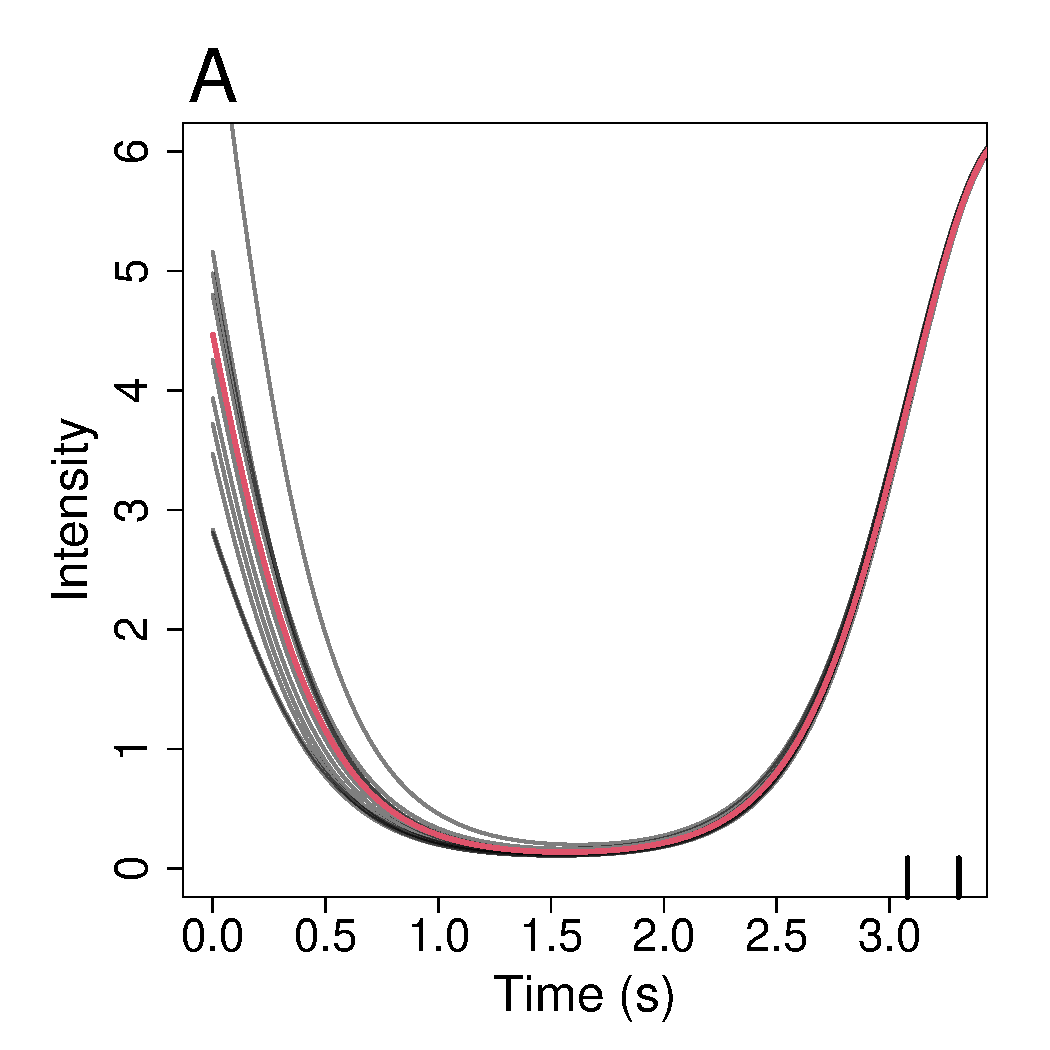
\includegraphics[width = 0.45\linewidth]{Current_1.pdf} }} \quad
      \subfloat{{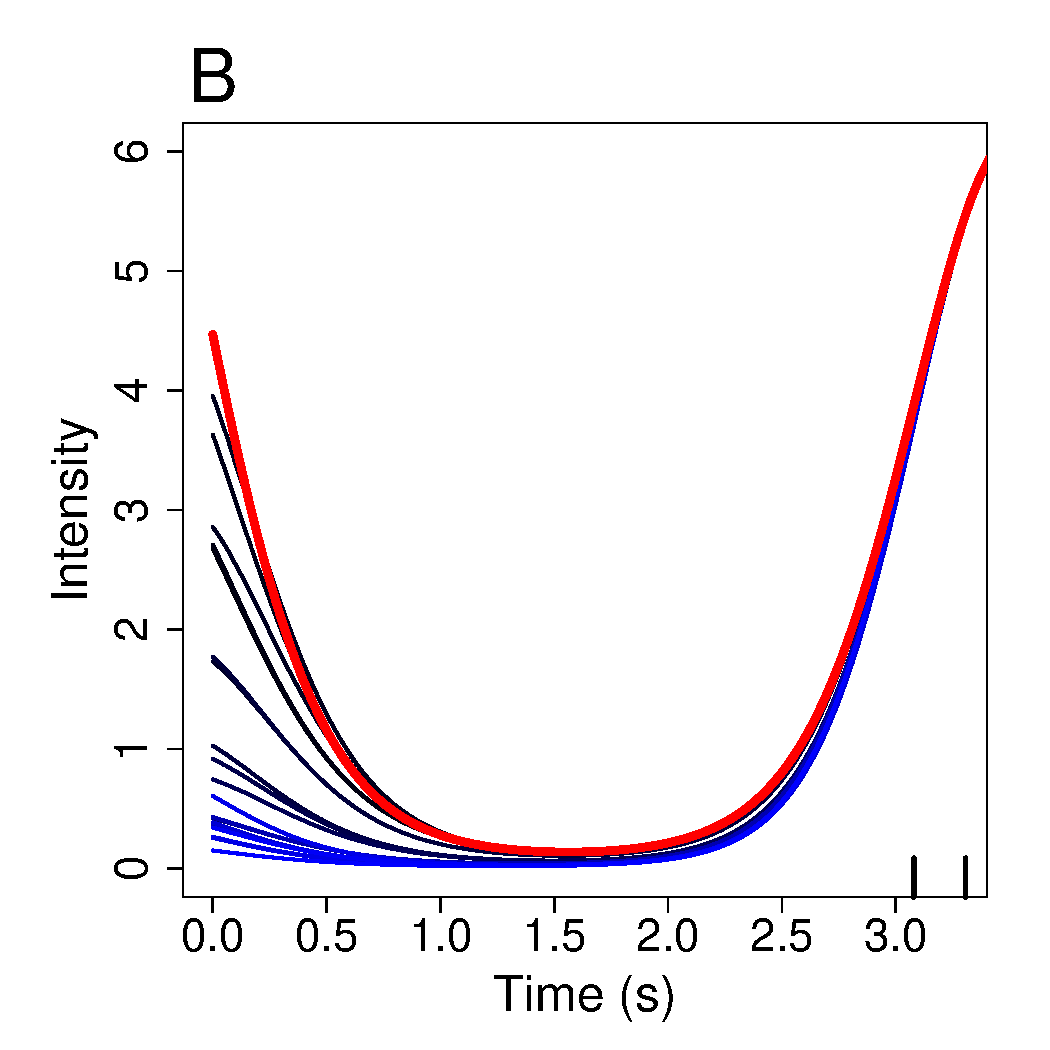
\includegraphics[width = 0.45\linewidth]{Current_2.pdf} }} 
    \end{center}     
    \caption{ Illustration of proposal mechanism when $f = \log \mathbf{x}_A$. (A) shows ten candidate functions --- grey lines --- where the current intensity is shown by the red line. (B) 100 iterations of the proposal mechanism where the original $\mathbf{x}_A$ is the red line. The iterations progress from black to blue. The black ticks show the spike times.}
    \label{fig:current}
    \hrulefill
    \end{figure}


 However, this approach may be slow at `flattening' the intensity in region $A$. This is because the candidate intensity functions are centered on $\mathbf{x}_A$. Therefore, we also propose both functions that have `steeper' intensity or `flatter' intensity in region $A$. This can be seen in Figure \ref{fig:current}(A) which shows ten candidate intensities --- with fixed partition --- zoomed in on the region $[0,3.3]$. The proposal parameters are $K=10$, $M=337$, $l = 1.59$, $\sigma_n^2 = 1e^{-5}$ and $\sigma^2 = 1$. The red line shows the current intensity function $\mathbf{x}_A$ and the grey lines show ten candidate intensity functions. We see that four of the candidate functions have larger intensity than $\mathbf{x}_A$ and the majority of proposals are close to $\mathbf{x}_A$. It is also important to note that the smaller $\mathbf{x}_A$ the more difficult it is to proposal smaller values since the calculations are done on the logarithmic scale. For example, suppose on the logarithmic scale the intensity at time $t$ is $0$ and the drawn candidate value equals $-1$, this translates to an original intensity of $1$ and candidate intensity equal $0.368$, hence squashing smaller values closer together. This implies that it will take many iterations to flatten the curve in the region $[0,1]$. Indeed, this is shown in Figure \ref{fig:current}(B) where the red line shows $\mathbf{x}_A$, we then compute $100$ iterations where $K=10$, $w=100$, $l = 1.59$, $\sigma_n^2 = 1e^{-5}$ and $\sigma^2 = 1$. The iterations are shown going from the black   lines to blue lines as iterations progress. We see that we do indeed steadily flatten the intensity function in the region $[0,1]$. 
 
 %Summary of f = current
 So we have found that using $f = f_{\mathrm{cur}}$ does reduce the peak intensity found at time $0$s. However, it often requires a large number of iterations to do this.  
 % Discuss the two alternatives
  With this in mind, it may be more intuitive to propose functions whose shape is flatter than the current intensity function. For example proposing intensity functions whose mean is constant.  We shall consider two alternative functions for $f$ both of which are constant. Namely, $f_{\mathrm{mean}} = \{\mathrm{mean}(\log \mathbf{x}_A)\}^M_{i=0}$ which returns the constant vector where each element is the mean of $\log \mathbf{x}_A$ and $f_{\mathrm{min}} = \{\mathrm{min}(\log \mathbf{x}_A)\}^M_{i=0}$ which returns the constant vector where each element is the minimum of $\log \mathbf{x}_A$. 
  
   \begin{figure}[t!]
   \begin{center} 
    \subfloat{{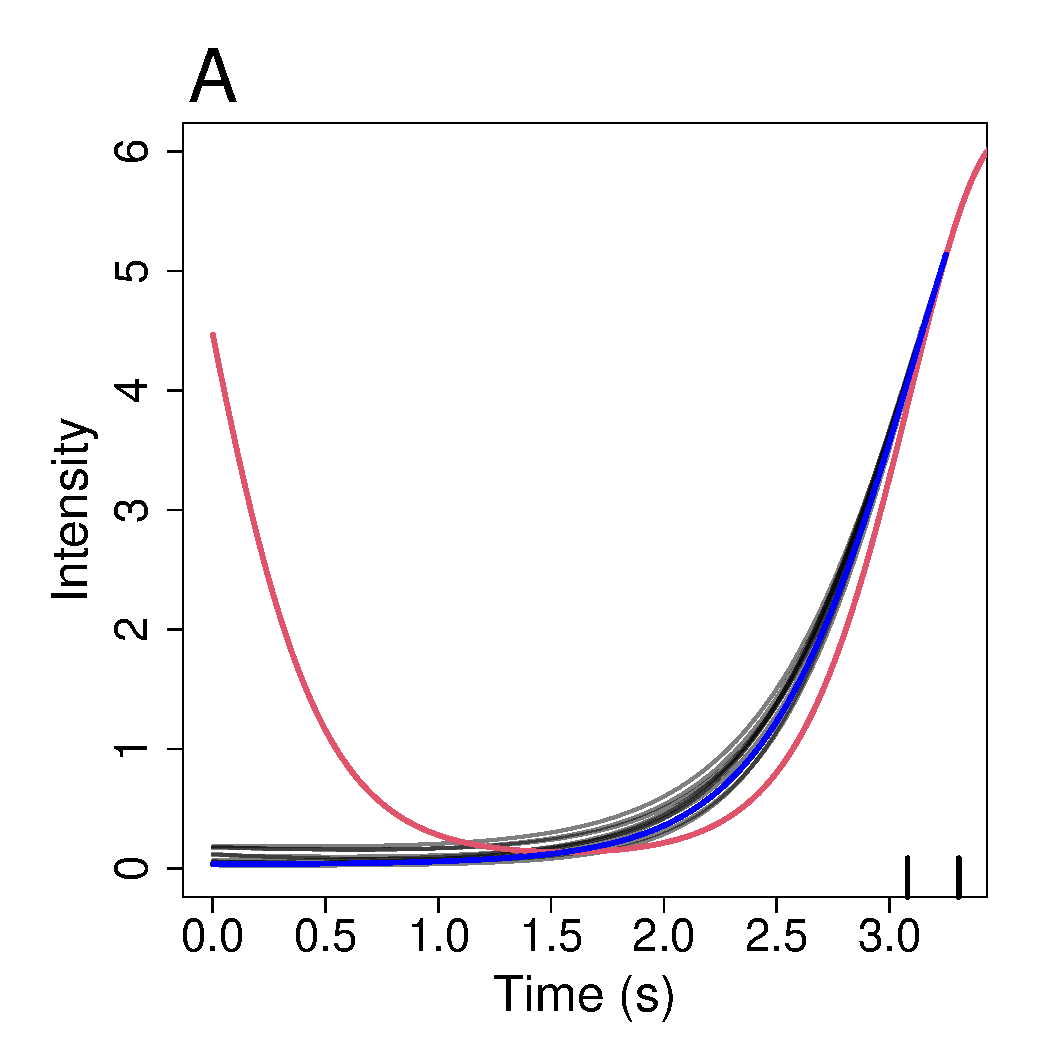
\includegraphics[width = 0.42\linewidth]{Min_1.pdf} }} 
      \subfloat{{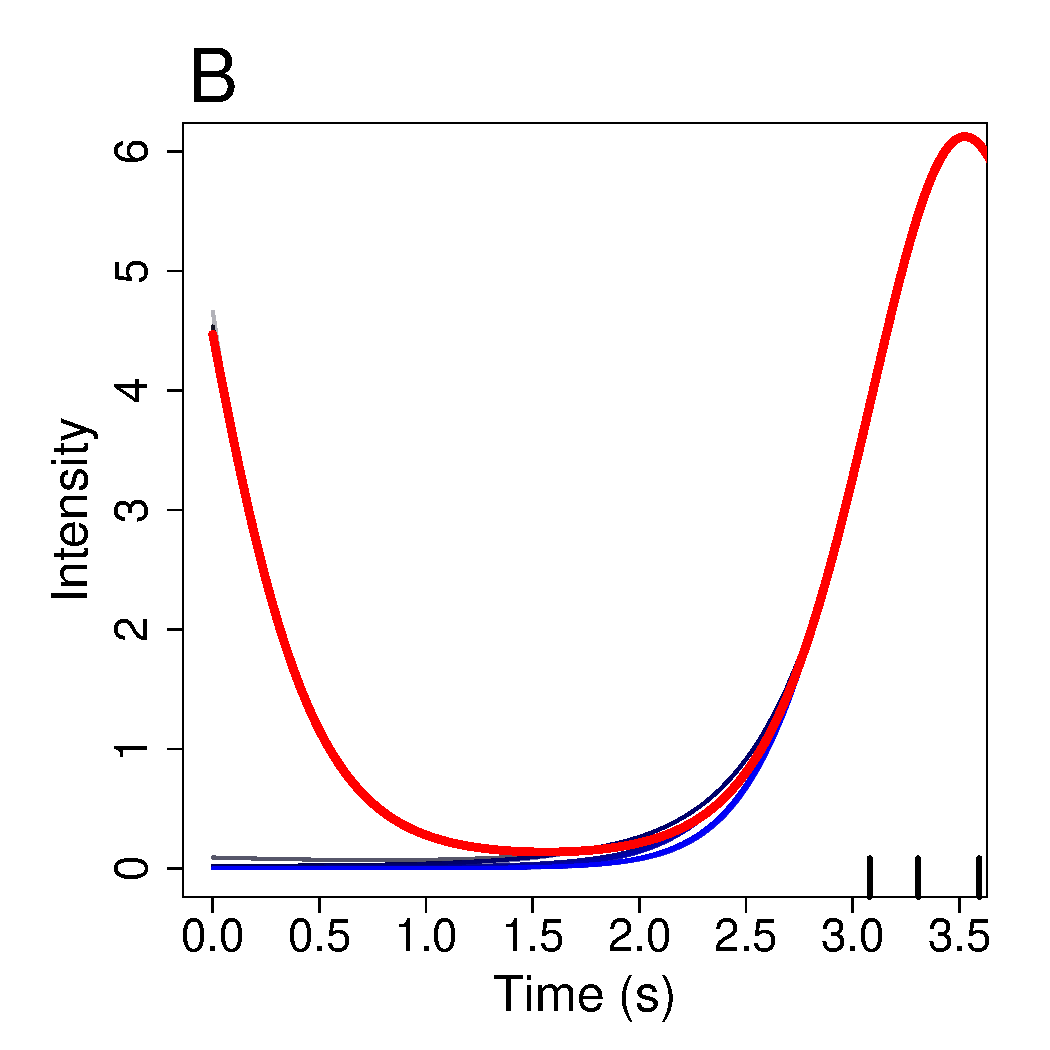
\includegraphics[width = 0.42\linewidth]{Min_2.pdf} }}\\
         \subfloat{{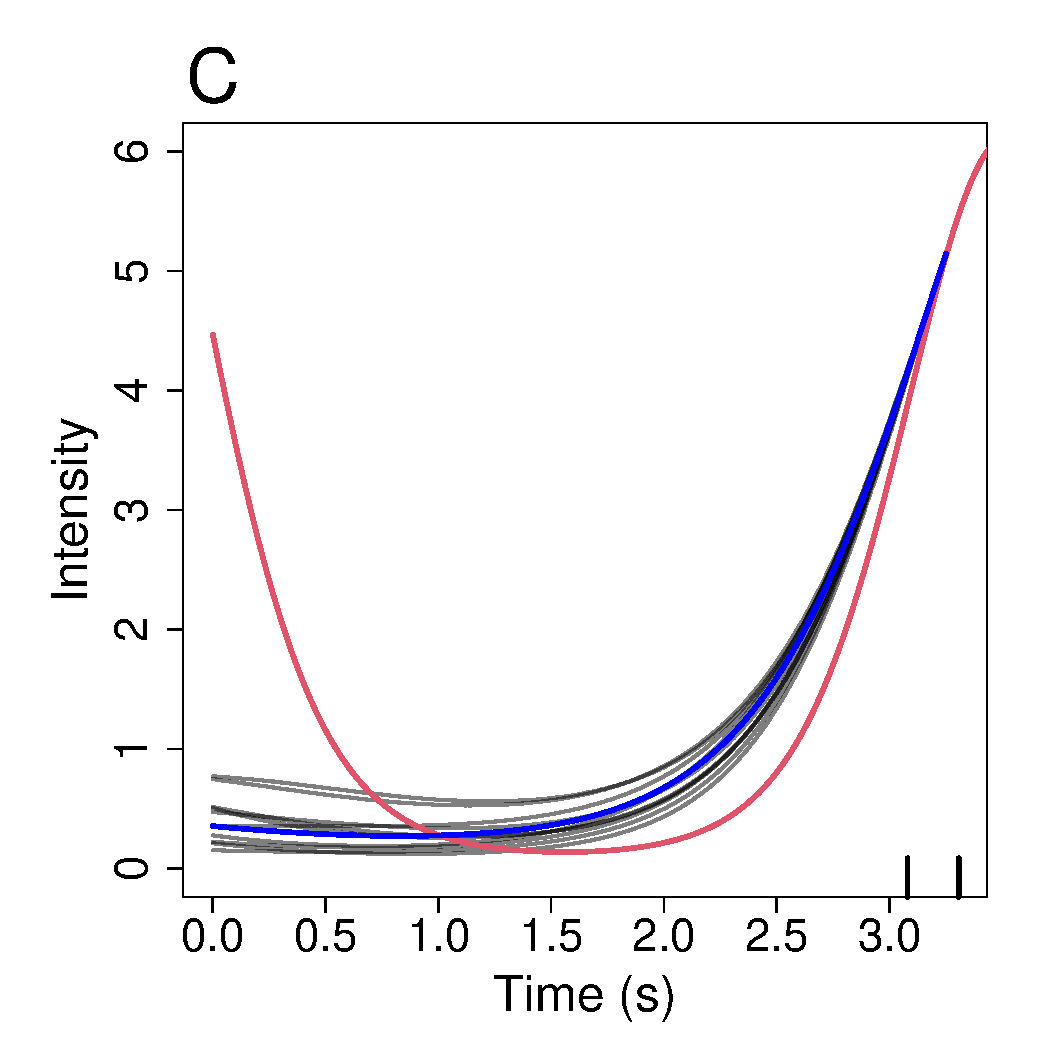
\includegraphics[width = 0.42\linewidth]{Mean_1.pdf} }}
      \subfloat{{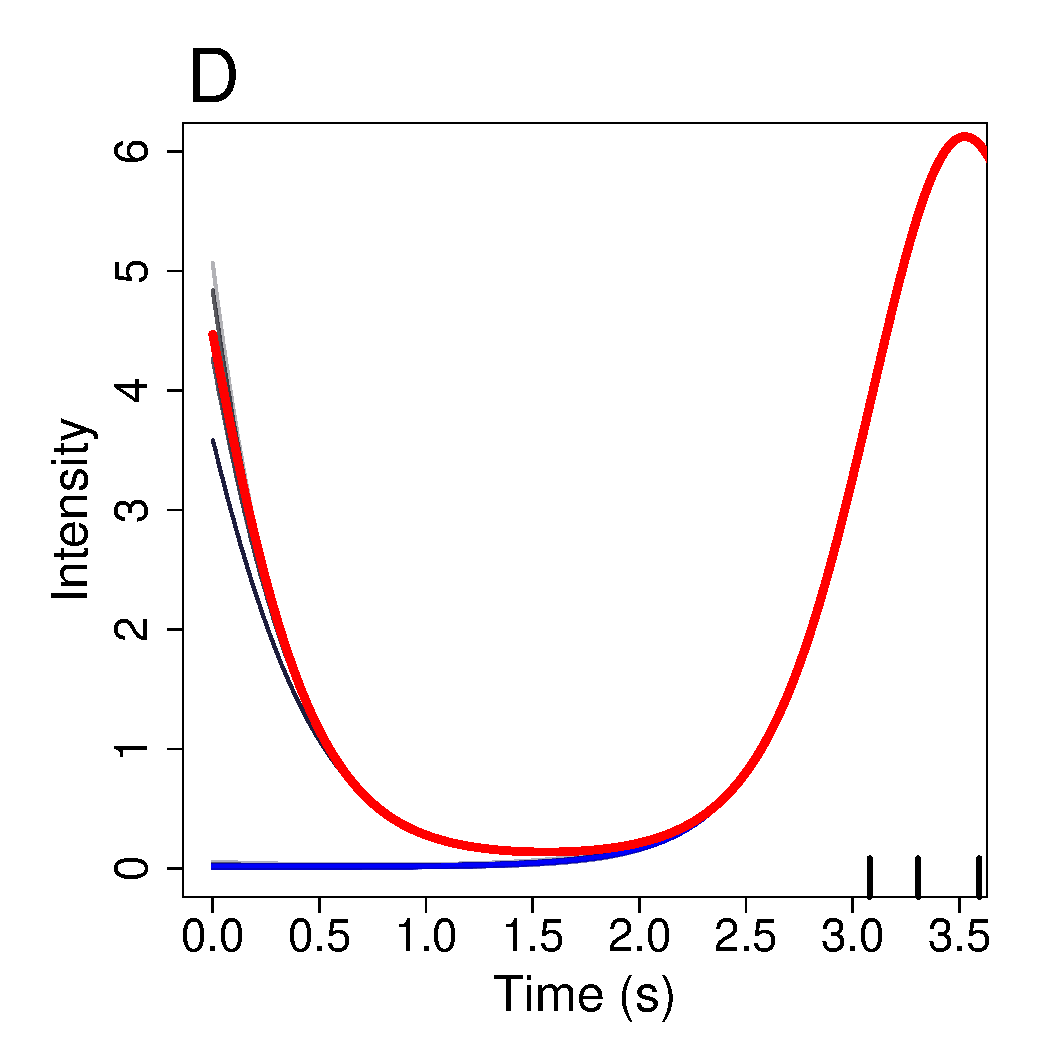
\includegraphics[width = 0.42\linewidth]{Mean_2.pdf} }} 
    \end{center}     
    \caption{Illustration of the mean of a MVN distribution where black shows the mean for the current version and also the current value of $\mathbf{x}_A$ red uses the mean and blue the min. (A-D) shows the results for different widths of region $A$ where the width gets wider as (A) goes to (D).}
    \label{fig:varyf}
    \hrulefill
    \end{figure}
    
  % Plot showing f_{\mathrm{min}} and f_{\mathrm{mean}} in action. 
  In Figures \ref{fig:varyf}(A) and (C) we show ten candidate functions from the proposal distribution using $f_{\mathrm{min}}$ and $f_{\mathrm{max}}$, respectively, where the blue lines show the mean of the proposal distribution. This illustrates how using $f_{\mathrm{min}}$ and $f_{\mathrm{max}}$ makes the candidate intensity functions flatter than those using $f = f_{\mathrm{cur}}$ in Figure \ref{fig:current}. For both the proposal parameters were $K=10$, $M=337$, $l = 1.59$, $\sigma_v^2 = 1e^{-5}$ and $\sigma^2 = 0.5$. Therefore, if accepted we require fewer iterations then $f_{\mathrm{cur}}$ to remove the peak intensity at time $0$. We also see a marginal difference between using $f_{\mathrm{mean}}$ and $f_{\mathrm{min}}$ where the proposed functions using $f_{\mathrm{min}}$ are smaller than those using $f_{\mathrm{mean}}$. In (B,D) we plot $100$ iterations of using this proposal mechanism, where we begin at the red line. Iterations are shown going from grey to blue lines at the iterations progress. We see that both options flatten the intensity, in a small iterations. For $f_{\mathrm{mean}}$ we see a couple iterations remain around the initial intensity before jumping to a flat intensity. This is because the width is small in the initial iterations--- for example corresponding to time 0.5 --- thus the proposed intensities remain high. However, it took $f_{\mathrm{min}}$ and $f_{\mathrm{mean}}$ 14 and 15 iterations, respectively, to accept a candidate function with a flat intensity in $[0,2]$. Therefore, we find that the acceptance probability is lower for $f_{\mathrm{mean}}$ and $f_{\mathrm{min}}$ compared to $f_{\mathrm{cur}}$. However, it takes $f_{\mathrm{cur}}$ far longer to propose functions with initial flat intensity. 
  
  %Discussion which f to use
  In the above discussion we have always used the same initial intensity function, and we found that all considered $f$ do reduce the high intensity found in the region $[0,1.5]$. Therefore when deciding which method to implement we are interested in the speed at which the proposals flatten this region. Therefore, in the particular example shown one would choose to use either $f_{\mathrm{min}}$ or $f_{\mathrm{mean}}$ as they took a similar amount of iterations. However, in general it can take a large number of iterations to accept a proposal when using $f_{\mathrm{min}}$ or $f_{\mathrm{mean}}$. For example in Figure \ref{fig:badCandidate} we show the mean of the proposal --- the red line --- compared to the current intensity function on the log scale. We see that the two lines differentiate by a large margin, and in this case the prior ratio stops candidate functions been accepted. In particular, the log prior ratio of the posterior mean against the current intensity is $-54.8$, which outweighs the log likelihood ratio of $1.08$. The mean of the proposal is decreases quickly because of the gradient of the values it is conditioned on.
  
   \begin{figure}[t]
   \hrulefill
   \begin{center} 
    \subfloat{{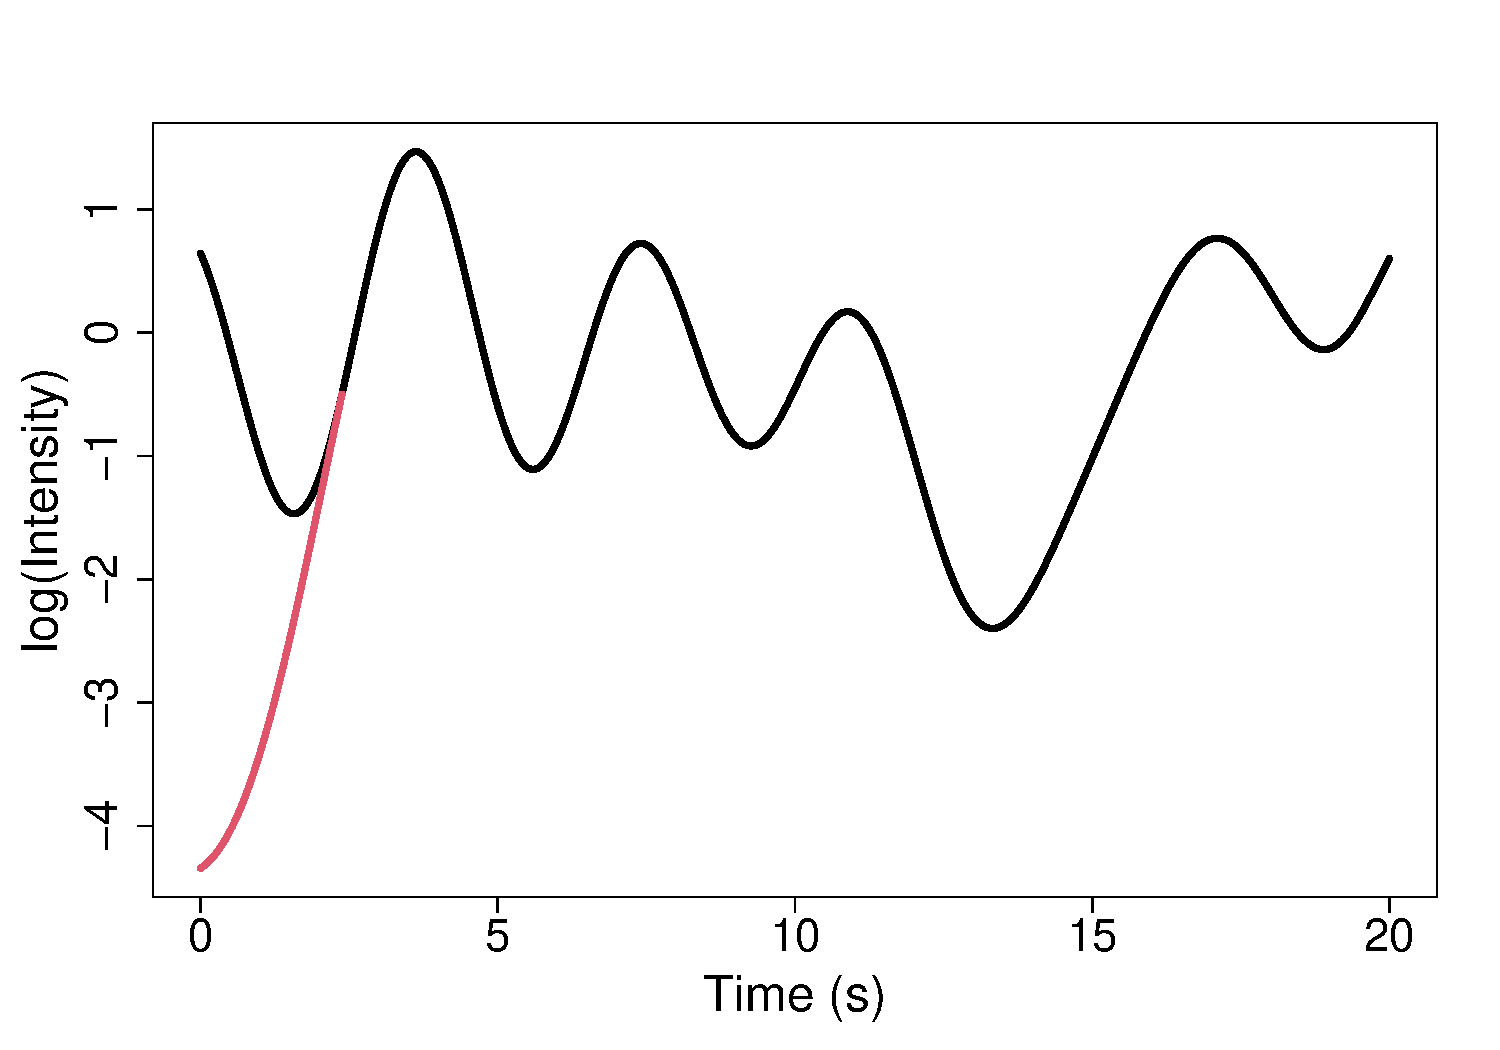
\includegraphics[scale = 0.5]{BadExample.pdf} }}
    \end{center}     
    \caption{Example where the mean of the proposal ---red line --- is far from  the current intensity on the logarithmic scale. }
    \label{fig:badCandidate}
    \hrulefill
    \end{figure}
    

  Therefore, we find that if candidate functions are accepted fast enough $f_{\mathrm{min}}$ and $f_{\mathrm{mean}}$ will flatten the region quicker. However, there is no guarantee that candidate functions will get accepted.   Thus, although $f_\mathrm{cur}$ reduces the intensity less per iteration it  will not get stuck not accepting proposals. 
  
  Other functions could be used in this proposal mechanism, and further research could look into whether there is an optimal $f$ for proposing updates to the intensity function on these regions of interest.   
  
  
  \subsection{Proposal mechanism for GP}
We now need to decide how to use this new proposal in conjunction with the under-relaxed method. We choose to use both $f_{\mathrm{cur}}$ and $f_{\mathrm{min}}$  because $f_{\mathrm{min}}$ can quickly flatten the intensity if accepted, and $f_{\mathrm{cur}}$ can reduce the intensity if $f_{\mathrm{min}}$ fails to. We only want to update on at the beginning and end of the function infrequently. This is because we are only using this method to help explore regions that the under-relaxed methods struggles to search. Therefore, we will only use this proposal every $1000$th iteration, but we shall use the proposal multiple times. This is to improve the chance of removing undesired features in these regions. We choose to initially do 50 iterations on both the beginning and end of the function using $f_{\mathrm{min}}$. %We use this method because if a candidate function is accepted then often no further iterations are required to remove the undesired features.
If no candidate functions are accepted under $f_{\mathrm{min}}$ then we do a further 50 iterations using $f_\mathrm{cur}$. The algorithm for the MCMC is shown in Algorithm \ref{algor:GPx}.

\begin{algorithm}[t]
\DontPrintSemicolon
\textbf{Input:} \text{Spikes, ISI distribution,  $T$, Numer of iterations $N_\mathrm{iter}$, $\mathbf{t}$, GP hyper parameters, ISI parameter } \\
\textbf{Output:} \text{M samples of intensity $\mathbf{x}$} \\
Set initial values $\mathbf{x}^{(0)}$; \; 
\For{$i$ in $1$ to ($M+M_\mathrm{burn}$)}{
 Propose $\mathbf{x}_{\mathrm{can}}$ and calculate acceptance probability using under-relaxed method, update $\mathbf{x}^{(i)}$; \;
\If{i \%\% 1000 == 0}{
\For{ j in $1$ to $50$}{
	Use conditional method at the start with $f_{\mathrm{min}}$, and conditional method at the end with $f_{\mathrm{min}}$ to update $\mathbf{x}^{(i)}$; \;
}
\If{No proposals using $f_{\mathrm{min}}$ are accepted}{
\For{ j in $1$ to $50$}{
	Use conditional method at the start with $f_{\mathrm{cur}}$, and conditional method at the end with $f_{\mathrm{cur}}$ to update $\mathbf{x}^{(i)}$;\;}}
}
}
\text{Return:} $\mathbf{x}$; 
\caption{Inference for GP intensity function.}
\label{algor:GPx}
\end{algorithm} 



      


\end{document}
